\documentclass[utf8, diplomski, numeric]{fer}
\usepackage{booktabs}
\usepackage[final]{pdfpages}
\usepackage{beramono}
\usepackage{subcaption}
\usepackage{listings}

\newcommand\keywordstyle[1]{{\bfseries{#1}}}%
\lstset{
    language=C,
    basicstyle=\small\ttfamily,
    numbers=left,
    numberstyle=\tiny,
    showstringspaces=false,
     morekeywords={definiraj, inicijaliziraj, za, ako, onda, dok, inače, inace, nastavi, ponavljaj},
     literate={đ}{{\dj}}1
          		{ž}{{\v{z}}}1
          		{č}{{\v{c}}}1
          		{ć}{{\'c}}1
          		{š}{{\v{s}}}1
          		{inače}{{\keywordstyle{ina\v{c}e}}}5,
  }

\renewcommand{\lstlistingname}{Pseudokod}

\begin{document}

% TODO: Navedite broj rada.
\thesisnumber{2981}

% TODO: Navedite naslov rada.
\title{Usporedba algoritama grupiranja u postupcima otkrivanja anomalija}

% TODO: Navedite vaše ime i prezime.
\author{Jelena Nemčić}

\maketitle

% Ispis stranice s napomenom o umetanju izvornika rada. Uklonite naredbu \izvornik ako želite izbaciti tu stranicu.

\includepdf[pages=-]{izvornik.pdf}

% Dodavanje zahvale ili prazne stranice. Ako ne želite dodati zahvalu, naredbu ostavite radi prazne stranice.
\zahvala{}

\tableofcontents

\chapter{Uvod}

Svaki dan generira se velika količina podataka koja se zatim obrađuje kako bi se iz nje saznale nove informacije. Jedan od načina korištenja podataka jest otkrivanje neobičnog ponašanja i pronalaženje anomalija.

Anomalijom se smatra svaki događaj ili opažanje koje značajno odstupa od većine podataka i ne ponaša se na očekivan način. Takvi primjeri mogu izazvati sumnju da ih generira drugačiji mehanizam ili se činiti nedosljednima s ostatkom tog skupa podataka.

Otkrivanje anomalija pronalazi primjenu u mnogim domenama uključujući kibernetičku sigurnost, medicinu, računalni vid, statistiku, neuroznanost i oružane snage. Koristi se također i za otkrivanje financijskih prijevara, industrijskih oštećenja i poremećaja u ekosustavu. Anomalije mogu predstavljati problem te su tada tražene radi namjernog izostavljanja iz skupa podataka kako bi se dobila točnija statistička analiza ili bolje predviđanje nekog modela strojnog učenja. Međutim, u mnogim su primjenama anomalije najzanimiljiviji dio skupa podataka i predstavljaju novu pojavu koju je potrebno identificirati i dalje istražiti.

Jedna od tehnika otkrivanja anomalija jest korištenje algoritama grupiranja s ciljem pronalaženja elemenata koji ne pripadaju niti jednoj grupi. U ovom radu dano je objašnjenje problema pronalaska anomalija, opis različitih algoritama grupiranja i korištenih skupova podataka te usporedba izvedbe tih algoritama u postupcima otkrivanja anomalija. Algoritmi odabrani za usporedbu su algoritam K-sredina, DBSCAN i Gaussova mješavina, a testirani su na problemima otkrivanja ...


\chapter{Anomalije}
\section{Pojava anomalija i njeni uzroci}
Postoji više pokušaja definiranja anomalija, a većina njih opisuje anomaliju kao opažanje čiji se obrazac ponašanja razlikuje od očekivanog, najčešće se pojavljuje vrlo rijetko u skupu podataka i njegova su obilježja značajno drugačije od onih većine preostalih opažanja. Također, anomalijom se može smatrati podatak koji se čini nedosljedan i relativno udaljen od drugih podataka iz skupa ili izaziva sumnju da ga generira drugačiji mehanizam.

Anomalije se mogu pojaviti u bilo kojem skupu podataka i ponekad njihovo otkrivanje može biti od izuzetne važnosti. Često se otkrivanje anomalija provodi u predobradi kako bi se mogle ukloniti iz skupa podataka. Time se dobiva točnija statistika podataka, bolje predviđanje modela strojnog učenja i bolja vizualizacija podataka. S druge strane, anomalije mogu biti najvažnija i najzanimljivija opažanja i tada se otkrivanje anomalija provodi radi njih samih. Primjeri takve primjene su otkrivanje upada u području kibernetičke sigurnosti, otkrivanje financijskih prijevara i lažnih informacija, otkrivanje kvarova i pogrešaka, praćenje stanja sustava i vremenskih serija, detekciju događaja u senzorskim mrežama, otkrivanje poremećaja u ekosustavu, otkrivanje nedostataka na slikama pomoću računalnog vida te za postavljanje medicinske dijagnoze i provođenje zakona.

Mogući uzroci pojave anomalija su:
\begin{enumerate}
\item Podaci pripadaju različitim razredima.
\begin{itemize}
\item Anomalije se razlikuju od ostalih podataka jer pripadaju drugom razredu, koji ima drugačija obilježja.
\item Primjer takvih anomalija su financijske prijevare, strani upad u sustav i pojava bolesti.
\end{itemize}

\item Prirodna varijacija.
\begin{itemize}
\item Neki skupovi podataka mogu se modelirati normalnom distribucijom, gdje su anomalije oni događaji koji imaju vrlo malu vjerojatnost pojavljivanja.
\end{itemize}

\item Pogreške u mjerenju ili prikupljanju podataka.
\begin{itemize}
\item Do pojave anomalija može doći ako podaci sadrže šum, ako postoji kvar u mjernim instrumentima ili zbog ljudske pogreške.
\item Krajnji je cilj eliminirati ovakve anomalije jer smanjuju kvalitetu podataka.
\end{itemize}

\end{enumerate}

U ovom radu razmatrat će se samo anomalije koje se javljaju kao posljedica toga što podaci prirodno pripadaju različitim razredima.


\section{Klasifikacija anomalija}
Kako bi sustav za otkrivanje anomalija mogao točno identificirati potencijalna odstupanja, nužno je znati koja vrsta anomalije se očekuje. Anomalije se mogu podijeliti u tri glavne kategorije:

\begin{enumerate}
\item Globalne anomalije

Opažanje se smatra globalnim odstupanjem ili globalnom anomalijom ako se njegova vrijednost ili vrijednost nekih njegovih obilježja značajno razlikuje od vrijednosti cjelokupnog skupa podataka. Gledano u n-dimenzionalnom prostoru, taj se podatak nalazi daleko od svih ostalih podataka iz skupa. Primjer globalne anomalije dan je na slici \ref{fig:outlier1}.

\begin{figure}[htb]
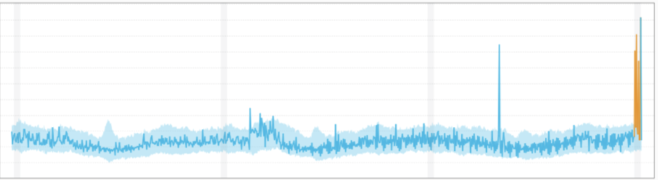
\includegraphics[width=1\textwidth]{images/outlier_type1.png}
\centering
\caption{Globalna anomalija. Preuzeto s  https://towardsdatascience.com/outliers-analysis-a-quick-guide-to-the-different-types-of-outliers-e41de37e6bf6}
\label{fig:outlier1}
\end{figure}

\item Kontekstualne anomalije

Kontekstualne ili uvjetne anomalije su opažanja čije se vrijednosti znatno razlikuju od ostalih opažanja koja postoje u istom kontekstu. Takve vrijednosti ne moraju biti izvan globalnih očekivanja, ali odudaraju od konteksta u kojem se nalaze. Također, jedan podatak koji je anomalija u kontekstu jednog skupa podataka ne mora biti anomalija u drugom. Ovakva odstupanja najčešća su u podacima vremenskih serija jer takvi skupovi podataka sadrže zapise ovisne o vremenskom razdoblju. Slika \ref{fig:outlier2} prikazuje primjer takve anomalije.

\begin{figure}[htb]
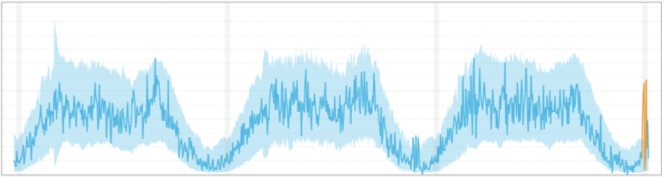
\includegraphics[width=1\textwidth]{images/outlier_type2.png}
\centering
\caption{Kontekstualna anomalija}
\label{fig:outlier2}
\end{figure}

\item Kolektivne anomalije

Podskup podataka smatra se kolektivnom anomalijom ako njihove vrijednosti kao grupa značajno odstupanju od cijelog skupa podataka, ali vrijednosti pojedinačnih podataka nisu same po sebi anomalne ni u globalnom niti u kontekstualnom smislu. U podacima vremenskih serija, kolektivne anomalije mogu se manifestirati kao vrhovi i doline koje se javljaju izvan vremenskog okvira kada je takvo ponašanje normalno, kao što se vidi na slici \ref{fig:outlier3}.

\begin{figure}[htb]
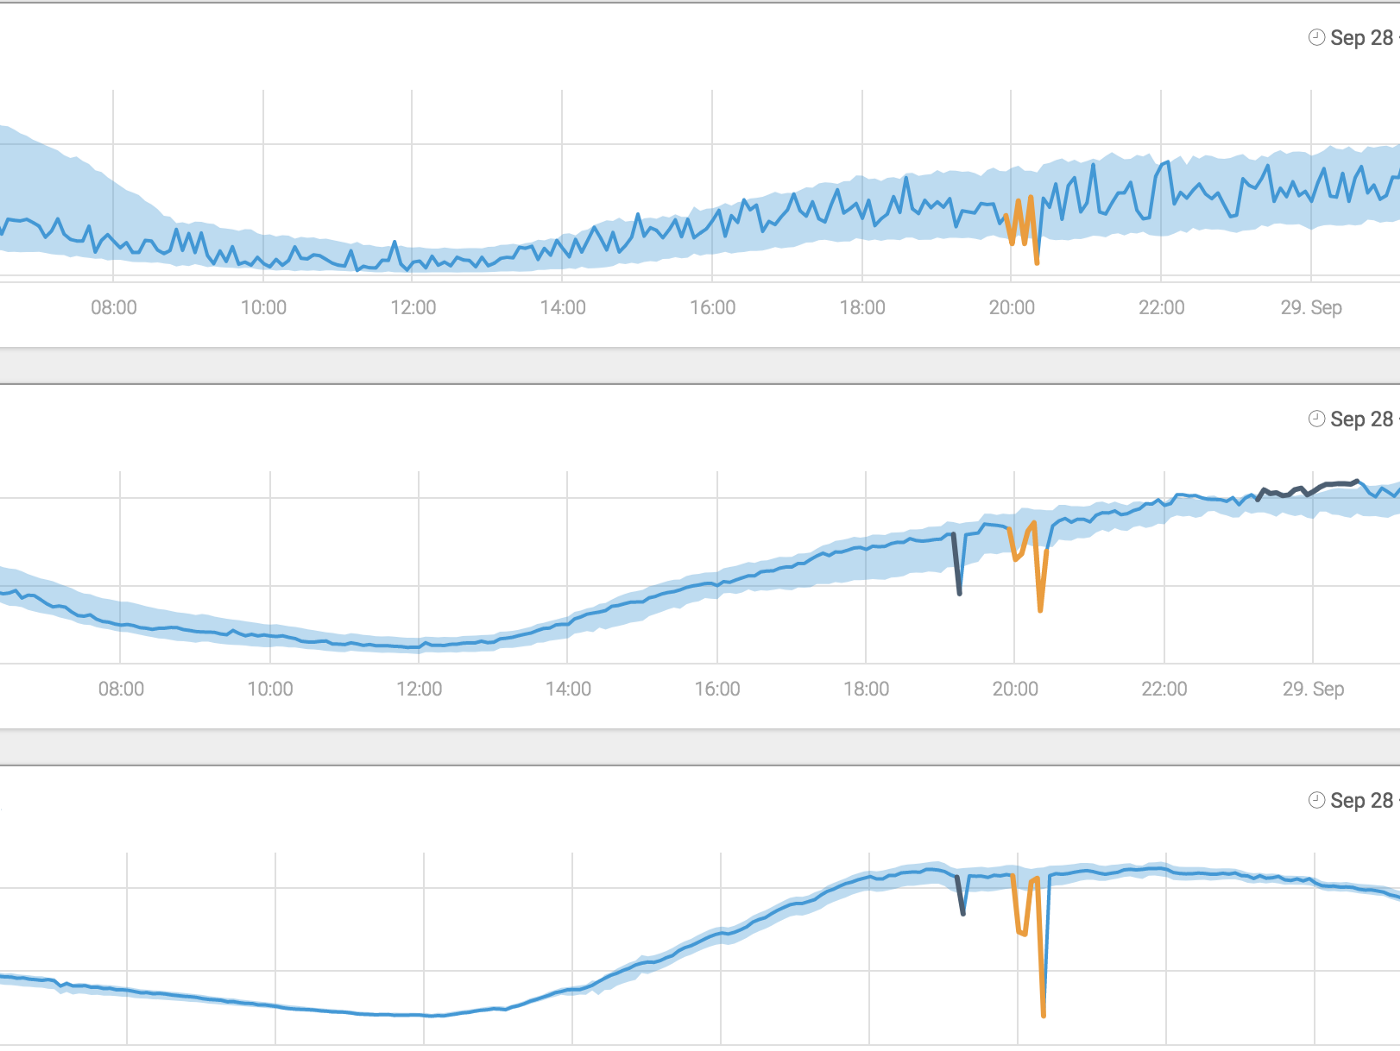
\includegraphics[width=1\textwidth]{images/outlier_type3.png}
\centering
\caption{Kolektivna anomalija}
\label{fig:outlier3}
\end{figure}

\end{enumerate}

Ovisno o vrsti anomalije primjenjuju se različite metode i načini detekcije. Ovaj rad fokusira se na globalne anomalije i njihovo pronalaženje.


\section{Problem otkrivanja anomalija}
Otkivanje anomalija svodi se na problem definiranja očekivanog ponašanja podataka ili granica unutar kojih se podaci smatraju normalnima te identificiranja točaka koje se ne nalaze unutar njih. Postoji nekoliko faktora koji čine ovaj problem vrlo teškim.

\begin{itemize}
\item Učinkovito modeliranje normalnih vrijednosti i ponašanja može biti vrlo izazovan problem. Često je teško nabrojati sva moguća normalna ponašanja nekog objekta i klasificirati neki podatak kao anomaliju. Također, granica  između normalnih podataka i anomalija može biti vrlo nejasna.
\item Svaki problem zahtjeva specifičan način detekcije anomalija jer su odabir mjere sličnosti i modeliranje odnosa ovisni o svojstvima tog problema. Zbog toga nije moguć razvoj univerzalno primjenjive metode otkivanja anomalija.
\item Prikupljeni podaci često sadrže šum koji može imati vrijednosti koje znatno odstupaju od normalnih ili čak nedostaju. Šum smanjuje kvalitetu podataka i otežava definiranje granica između normalnih podataka i anomalija te se često šum može pogrešno identificirati kao anomalija i obrnuto.
\item Mnogi načini otkrivanja anomalija postaju neučinkoviti u slučaju velike dimenzionalnosti skupa podataka. Podaci su tada rijetki i udaljenosti među podacima su sve veće te se puno točaka može pogrešno klasificirati kao anomalija.
\item U nekim primjenama, korisnik ne želi samo identificirati anomalije već i razumjeti zašto su ti podaci detektirani kao abnormalni. Zbog toga metoda otkrivanja anomalija mora biti razumljiva, smislena i pružiti opravdanje detekciji.
\end{itemize}


\section{Metode otkrivanja anomalija}
Postoji puno različitih tehnika otkrivanja anomalija i one se mogu podijeliti u četiri glavne kategorije.

\begin{enumerate}
\item Statističke metode

Statistički pristup naziva se još i pristup temeljen na modelu jer sadrži model koji opisuje obilježja skupa podataka. Model najčešće sadrži distribuciju vjerojatnosti podataka i za svaki podatak računa se vjerojatnost njegova pojavljivanja u tom modelu. Ako je ta vjerojatnost vrlo mala, podatak se proglašava anomalijom.
\item Metode temeljene na blizini
\begin{enumerate}
\item Metode temeljene na udaljenosti

Metode temeljene na udaljenosti pretpostavljaju da je podatak anomalija ako mu se najbliži susjedi nalaze daleko u prostoru značajki odnosno ako blizina objekta njegovim susjedima značajno odstupa od blizine većine drugih objekata njihovim susjedima u istom skupu podataka.
\item Metode temeljene na gustoći

Metode temeljene na gustoći koriste broj podataka koji se nalaze unutar definiranog prostora ispitivanog podatka za definiranje lokalne gustoće. Što je lokalna gustoća objekta manja, veća je vjerojatnost da je on anomalija.
\end{enumerate}
\item Metode temeljene na grupiranju

Metode koje se temelje na grupiranju pretpostavljaju da normalni podaci pripadaju velikim i gustim grupama, dok anomalije pripadaju malim i rijetkim grupama ili ne pripadaju niti jednoj. Razlika između grupiranja i metoda temeljenih na gustoći je u tome što grupiranje dijeli podatke u grupe dok metode temeljene na gustoći dijele podatkovni prostor.
\end{enumerate}
U ovom radu za detekciju anomalija koristit će se algoritmi temeljeni na grupiranju. Za usporedbu su izabrani algoritmi K-sredina, DBSCAN i Gaussova mješavina.


\chapter{Algoritmi grupiranja}
\section{O algoritmima grupiranja}
Grupiranje je podjela skupa podataka u grupe, tako da su podaci u istoj grupi sličniji jedni drugima nego podacima iz ostalih grupa. Cilj jest pronalaženje intrinzičnih grupa u skupu podataka. Algoritmi grupiranja pripadaju u skupinu nenadziranih metoda strojnog učenja jer su ulazni podaci dani bez ciljnih vrijednosti odnosno nisu označeni. 

\subsection{Podjela}
Grupiranje se može podijeliti u dvije kategorije:

\begin{enumerate}
\item Tvrdo grupiranje - podatak ili pripada grupi ili ne pripada
\item Meko grupiranje - podatak pripada svakoj grupi s određenom vjerojatnošću
\end{enumerate}

Osim po tipu grupiranja koje provode, algoritmi grupiranja razlikuju se i po tome kako definiraju pojam grupe i sličnost podataka. Svaki algoritam pretpostavlja specifičan model grupe, a najčešći modeli su:

\begin{enumerate}
\item Modeli povezanosti - na temelju udaljenosti podataka stvara se hijerarhijsko stablo grupa 
\item Centroidni modeli - podaci se organiziraju u nehijerarhijske grupe ovisno o udaljenosti od centroida te grupe
\item Modeli distribucije - grupe se modeliraju pomoću vjerojatnosti da podaci pripadaju istoj statističkoj distribuciji
\item Modeli gustoće - područja veće gustoće povezuju se u grupe
\end{enumerate}

Ne postoji objektivno najbolji algoritam grupiranja, već odabir algoritma ovisi o problemu koji se rješava. Algoritam se može odabrati na temelju modela grupe ili eksperimentalno. Također, algoritam dizajniran za jednu vrstu modela grupe općenito neće raditi na skupu podataka koji sadrži drugačiji tip grupa.

U ovom radu uspoređivat će se tri različita modela: algoritam K-sredina kao predstavnik centroidnih modela, DBSCAN algoritam kao model gustoće i model Gaussove mješavine koji pripada modelima distribucije.

\subsection{Vrednovanje}
Rezultati algoritama grupiranja mogu se vrednovati na dva načina. Prvi je vredovanje korištenjem podataka za koje su poznate oznake grupa. Takva evaluacija mjeri koliko je dobiveno grupiranje blizu unaprijed određenoj podjeli. Metode vrednovanja često su prilagođene varijante metoda koje se koriste za vrednovanje klasifikacije. Neke od tih metrika su:

\begin{enumerate}
\item Matrica zabune (eng. \textit{Confusion Matrix})

Matrica koja opisuje uspješnost modela prikazom broja istinski pozitivnih (eng. \textit{True Positive - TP}), lažno positivnih (eng. \textit{False Positive - FP}), istinski negativnih (eng. \textit{True Negative - TN}) i lažno negativnih (eng.  \textit{False Negative - FP}) primjera.
\item Točnost (eng. \textit{Accuracy})

Točnost je udio točno klasificiranih primjera u skupu svih primjera i računa se kao:
\begin{equation*} \label{eq:accuracy}
Acc = \frac{TP+TN}{TP+TN+FP+FN}
\end{equation*}

\item Preciznost (eng. \textit{Precision})

Preciznost predstavlja udio točno klasificiranih primjera među onima koje je model deklarirao kao pozitivne.
\begin{equation*} \label{eq:precision}
P = \frac{TP}{TP+FP}
\end{equation*}

\item Odziv (eng. \textit{Recall})

Odziv je udio točno klasificiranih primjera u skupu svih stvarno pozitivnih primjera.
\begin{equation*} \label{eq:recall}
R = \frac{TP}{TP+FN}
\end{equation*}

\item F1-mjera (eng. \textit{F1-score})

F1-mjera jest harmonijska sredina preciznosti i odziva i najčešće korištena mjera za usporedbu klasifikatora.
\begin{equation*} \label{eq:f1}
F1 = \frac{2PR}{P+R}
\end{equation*}

\item AUC mjera

ROC krivulja (eng. \textit{Receiver Operating Characteristic curve}) jest graf koji prikazuje odnos stope istiniski pozitivnih primjera (eng. \textit{True Positive Rate - TPR}) odnosno odziva i stope lažno pozitivnih primjera (eng. \textit{False Positive Rate - FPR}), koja se računa kao: 
\begin{math}
\frac{FP}{FP+TN}
\end{math}. Njihov odnos prikazuje se na svim mogućim pragovima klasifikacije. AUC mjera (eng. \textit{Area under the ROC curve}) predstavlja površinu ispod cijele ROC krivulje.

\end{enumerate}

Drugi način vrednovanja algoritama grupiranja jest korištenje metrika koje ne zahtjevaju oznake podataka kako bi izračunale efikasnost algoritma. Najčešće korištene metrike su:

\begin{enumerate}
\item Koeficijent siluete (eng. \textit{Silhouette Coefficient})

Koeficijent siluete definira se na temelju udaljenosti unutar grupe i između različitih grupa i računa se kao:
\begin{equation*} \label{eq:silouette}
S = \frac{1}{N}\sum_{i=0}^{N}\frac{b_i-a_i}{max(a_i,b_i)} 
\end{equation*}
gdje je:
\begin{itemize}
\item \textit{a} - srednja udaljenost između uzorka \textit{i} i svih ostalih podataka u toj grupi
\item \textit{b} - srednja udaljenost između uzorka \textit{i} i svih ostalih podataka u drugoj najbližoj grupi
\end{itemize}

Vrijednost koeficijenta siluete nalazi se u skupu \begin{math}[-1,1] \end{math} i što je ona veća, grupe su jasnije odijeljene i grupiranje se smatra točnijim.

\item Dunnov indeks

Dunnov indeks zahtjeva da su udaljenosti primjera unutar grupe male, a udaljenosti između različitih grupa što veće. Računa se kao:
\begin{equation*} \label{eq:silouette}
D = \frac{\min_{1\leq i < j \leq m} \delta(C_i,C_j)}{\max_{1\leq k \leq m} \Delta_k}
\end{equation*}
gdje je:
\begin{itemize}
\item $\delta(C_i,C_j)$ - udaljenost između grupa $C_i$ i $C_j$ (udaljenost između dva najbliža primjera, dva najudaljenija primjera ili prosječna udaljenost)
\item $\Delta_k$ - udaljenost primjera unutar iste grupe (najveća udaljenost između dva primjera, prosječna udaljenost ili udaljenost primjera od centroida grupe)
\end{itemize}

Što je vrijednost Dunnovog indeksa veća, bolje je grupiranje.

\item Davies Bouldin indeks

Davies Bouldin indeks računa se kao prosjek sličnosti svake grupe s grupom koja joj je najsličnija: 
\begin{equation*} \label{eq:silouette}
DB = \frac{1}{K}\sum_{i = 1}^{K} \max_{j\neq i} \frac{\Delta_i + \Delta_j}{\delta(C_i,C_j)}
\end{equation*}

Razlikuje se od ostalih metrika jer manja vrijednost ovog indeksa označava bolje grupiranje.

\item Randov indeks

\end{enumerate}

Za evaluaciju algoritama u ovom radu koristit će se sve navedene metode osim točnosti koja je nepouzdana u slučaju neuravnoteženih razreda, kao što je to slučaj u detekciji anomalija.

\section{K-sredine}
Algoritam K-sredina najpoznatiji je algoritam grupiranja koji se temelji na centroidnom modelu. U ovom algoritmu, svaka grupa ima centroid koji se računa kao srednja vrijednost članova grupe i predstavlja tu grupu. Primjeri se iz neoznačenog skupa podataka grupiraju u $K$ grupa na način da svaki podatak pripada onoj grupi čijem je centroidu najbliži. 

Kriterijska funkcija algoritma grupiranja jest funkcija koju taj algoritam nastoji minimizirati. Za algoritam K-sredina to je funkcija koja zbraja euklidske udaljenosti odstupanja primjera od centroida grupe u kojoj se nalaze i glasi:
\begin{equation*} \label{eq:silouette}
J = \sum_{k = 1}^{K}\sum_{x \in C_k} \lVert x - \mu_k \rVert ^{2}
\end{equation*}

Algoritam očekuje broj grupa $K$ kao hiperparameter i njegova se vrijednost može odrediti na više načina, a najpoznatiji su:
\begin{itemize}
\item Metoda lakta (eng. \textit{Elbow method})

U metodi lakta grafički se prikazuje ovisnost funkcije gubitka o broju grupa $K$. S porastom broja grupa vrijednost funckije će se smanjivati te je cilj pronaći ``lakat'' funkcije, odnosno broj grupa nakon kojeg se vrijednosti funkcija počinju smanjivati vrlo sporo.

\item Analiza siluete (eng. \textit{Silhouette analysis})

Ova je metoda grafička metoda koja se temelji na ranije objašnjenom koeficijentu siluete. Njegova vrijednost prikaže se za svaki primjer iz skupa podataka ovisno o grupi u koju je primjer raspoređen te se izabere onaj broj grupa za koji svi primjeri imaju približno jednak koeficijent siluete.

\end{itemize}

Osim odabira broja grupa, potrebno je definirati i način odabira početnih centroida. Neki od mogućih prisupa su:
\begin{itemize}
\item Nasumičan odabir $K$ primjera.
\item Nasumična dodjela grupe svakom primjeru i izračun centroida na temelju primjera u grupi.
\item Izračun srednje vrijednosti sviju primjera i dodavanje $K$ slučajnih vektora toj vrijednosti.
\item Nasumičan odabir prvog centroida, nakon čega se svaki sljedeći bira na način da bude što dalje od postojećih. Verzija algoritma koja implementira ovakav pristup zove se \textit{K-sredine++}.

\end{itemize}

Postupak grupiranja algoritma K-sredina je iterativan. Nakon inicijalizacije početnih centroida, svi se primjeri stavljaju u onu grupu čiji im je centroid najbliži. U sljedećem se koraku, na temelju razvrstanih primjera, ponovno računaju novi centroidi za svaku grupu. Dalje se ponavljaju ova dva koraka sve do konvergencije odnosno do trenutka kad više nema promjene u podjeli primjera grupama i u vrijednostima centroida. Ovaj postupak prikazan je i pseudokodom \ref{alg:kmeans}.

 \begin{lstlisting}[caption = Pseudokod algoritma K-sredina, label = {alg:kmeans}, escapeinside={*}{+}]
 definiraj broj grupa *$K$+
 inicijaliziraj centroide *$\mu_k$+, *$k = 1, ..., K$+
 ponavljaj
 	za svaki *$x_i \in D$+
 		pronađi najbliži centroid
 		dodjeli *$x_i$+ toj grupi
	za svaki *$\mu_k$+, *$k = 1, ..., K$+
		ažuriraj vrijednost centroida
 dok svi *$\mu_k$+ ne konvergiraju
\end{lstlisting}

Bitna karakteristika algoritma K-sredina je da pripada algoritmima tvrdog grupiranja, što znači da će svaku točku dodijeliti jednoj i točno jednoj grupi. Algoritam se dobro nosi s velikim skupovima podataka jer ima linearnu vremensku složenosti $O(nkdi)$, gdje je:
\begin{itemize}
\item n - veličina skupa podataka
\item k - broj grupa
\item d - dimenzionalnost podataka
\item i - broj iteracija algoritma
\end{itemize}

Međutim, algoritam K-sredina uvijek traži grupe sfernog oblika te ne može identificirati nekonveksne grupe. Također, jako je osjetljiv na prisutnost anomalija i šuma u podacima.

\section{DBSCAN}
DBSCAN algoritam (eng. \textit{Density-based spatial clustering of applications with noise}) priprada u skupinu algoritama grupiranja temeljenih na gustoći. On grupira zajedno točke koje su blizu jedna drugoj odnosno točke s mnogo susjednih točaka. Primjere koji nisu svrstani niti u jednu grupu i nalaze se u područjima niske gustoće algoritam označava kao anomalije. Kao i algoritam K-sredina, i DBSCAN je algoritam tvrdog grupiranja.

Glavna ideja algoritma DBSCAN jest da grupa mora sadržavati određeni minimalni broj točaka unutar definiranog polumjera. Zato algoritam zahtjeva dva parametra: 
\begin{enumerate}
\item \textit{minPts} 

Parametar \textit{minPts} predstavlja najmanji broj točaka u grupi da bi se ona smatrala gusto popunjenom. Za njegovu procjenu može se primjeniti generalno pravilo $minPts \geq D + 1$, gdje je $D$ broj dimenzija skupa podataka. Također, što je veći skup podataka potrebno je odabrati veći \textit{minPts} i tada se može koristiti pravilo $minPts = 2*D$. Veće vrijednosti obično daju bolje rezultate kada je u podacima prisutan šum.
\item $\epsilon$

Parametar $\epsilon$ jest polumjer unutar kojeg se traže susjedne točke. Pri odabiru vrijednosti $\epsilon$ nema generalnog pravila. Vrijednost ne smije biti ni prevelika niti premala i mora biti u skladu s udaljenostima među podacima. 
\end{enumerate}

DBCAN algoritam pridjeljuje svakoj točki jednu od tri moguće oznake:
\begin{enumerate}
\item Središnja točka (eng. \textit{Core point}) - točka oko koje se nalazi minimalno \textit{minPts} drugih točaka u polumjeru $\epsilon$
\item Granična točka (eng. \textit{Border point}) - točka koja ima barem jednu središnju točku na udaljenosti manjoj od $\epsilon$, ali nalazi se na rubu grupe i broj točaka oko nje manji je od \textit{minPts} 
\item Točka šuma (eng. \textit{Noise point}) - točka koja nije niti središnja niti granična točka; nije nužno anomalija, već samo točka od koje DBSCAN nije znao formirati grupu
\end{enumerate}

Na slici \ref{fig:dbscan-points} prikazane su grafički različite vrste točaka.

\begin{figure}[htb]
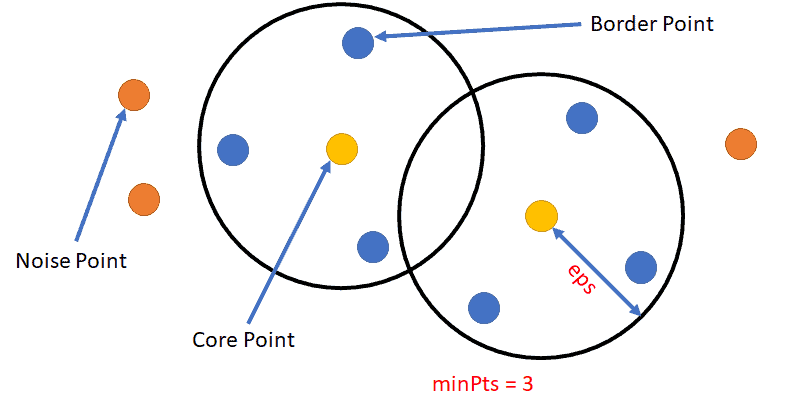
\includegraphics[width=0.8\textwidth]{images/dbscan-points.png}
\centering
\caption{Primjer središnje točke, granične točke i točke šuma uz $minPts$ = 3. Preuzeto s  https://machinelearninggeek.com/dbscan-clustering/}
\label{fig:dbscan-points}
\end{figure}

Središnja točka $p$ formira grupu zajedno sa svim središnjim i graničnim točkama koje su iz nje dohvatljive. Točka $q$ može biti:
\begin{itemize}
\item Izravno dohvatljiva - ako se nalazi unutar udaljenosti $\epsilon$ od točke $p$
\item Dohvatljiva - ako postoji put $p_1, ..., p_n$, pri čemu je $p_1 = p$ i $p_n = q$ i svaka točka $p_{i+1}$ izravno je dohvatljiva iz točke $p_i$
\end{itemize}

Dohvatljivost nije simetrična relacija, već samo središnje točke mogu dohvatiti granične. Zbog toga je uveden pojam povezanosti, kojim se formalno definira opseg grupe. Dvije točke $p$ i $q$ povezane su ako postoji točka $o$ takva da su i $p$ i $q$ dohvatljive iz $o$. Ova relacija je simetrična i grupa tada zadovoljava sljedeća svojstva:
\begin{itemize}
\item Sve točke unutar grupe međusobno su povezane.
\item Ako je točka dohvatljiva iz bilo koje točke koja pripada grupe, tada ona također pripada grupi.
\end{itemize}

Svojstva izravne dohvatljivosti, dohvatljivosti i povezanosti prikazana su grafički na slici \ref{fig:dbscan-dohvatljivost}.

\begin{figure}[htp]
\begin{subfigure}{.3\textwidth}
\centering
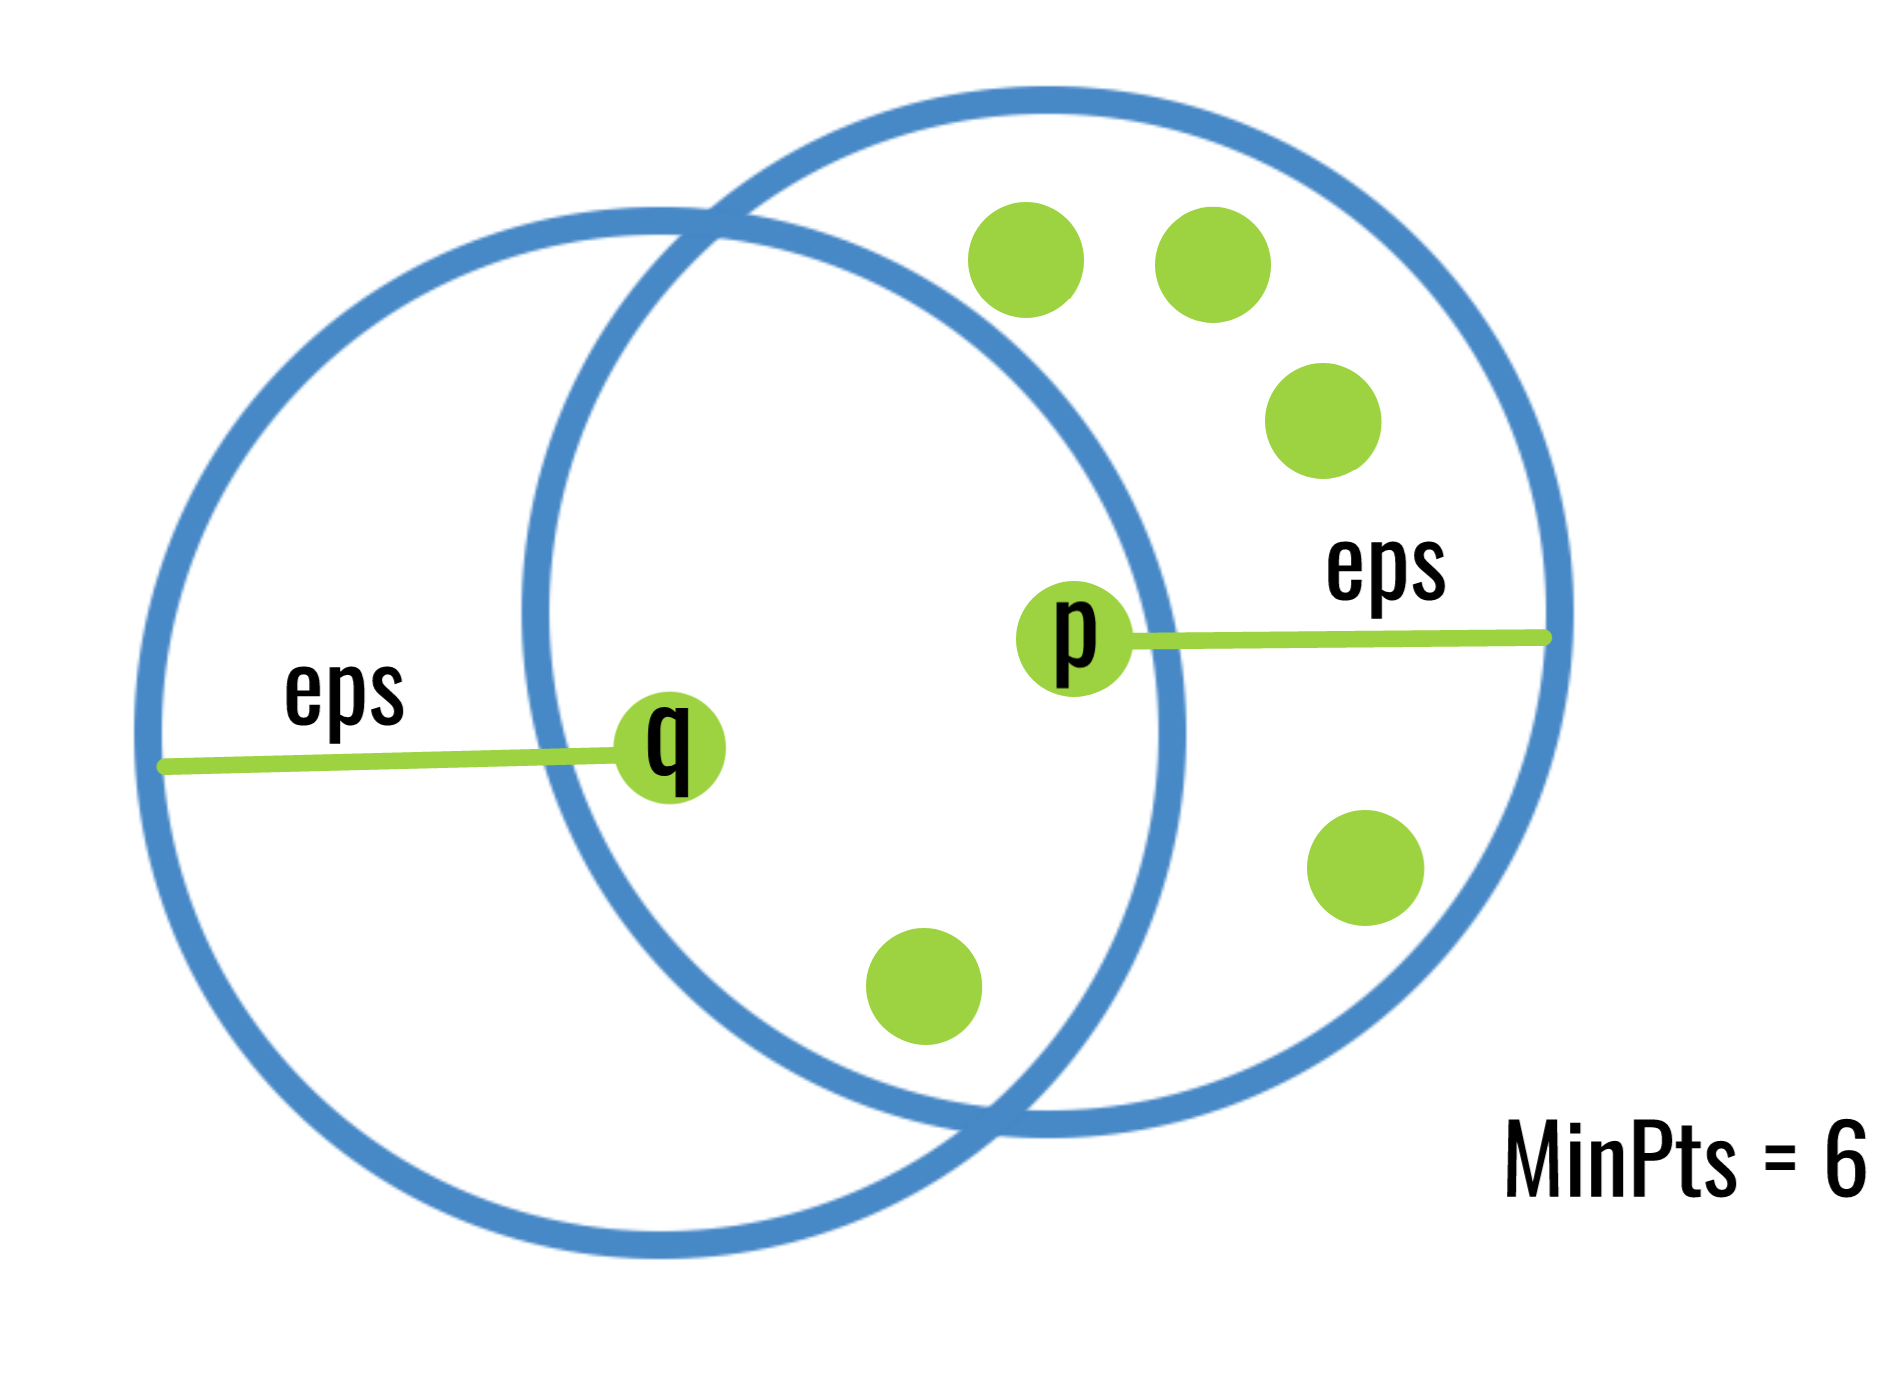
\includegraphics[width=1\textwidth]{images/dbscan1.png}
\caption{Točka $q$ je izravno dohvatljiva iz točke $p$}
\end{subfigure}
\begin{subfigure}{.3\textwidth}
\centering
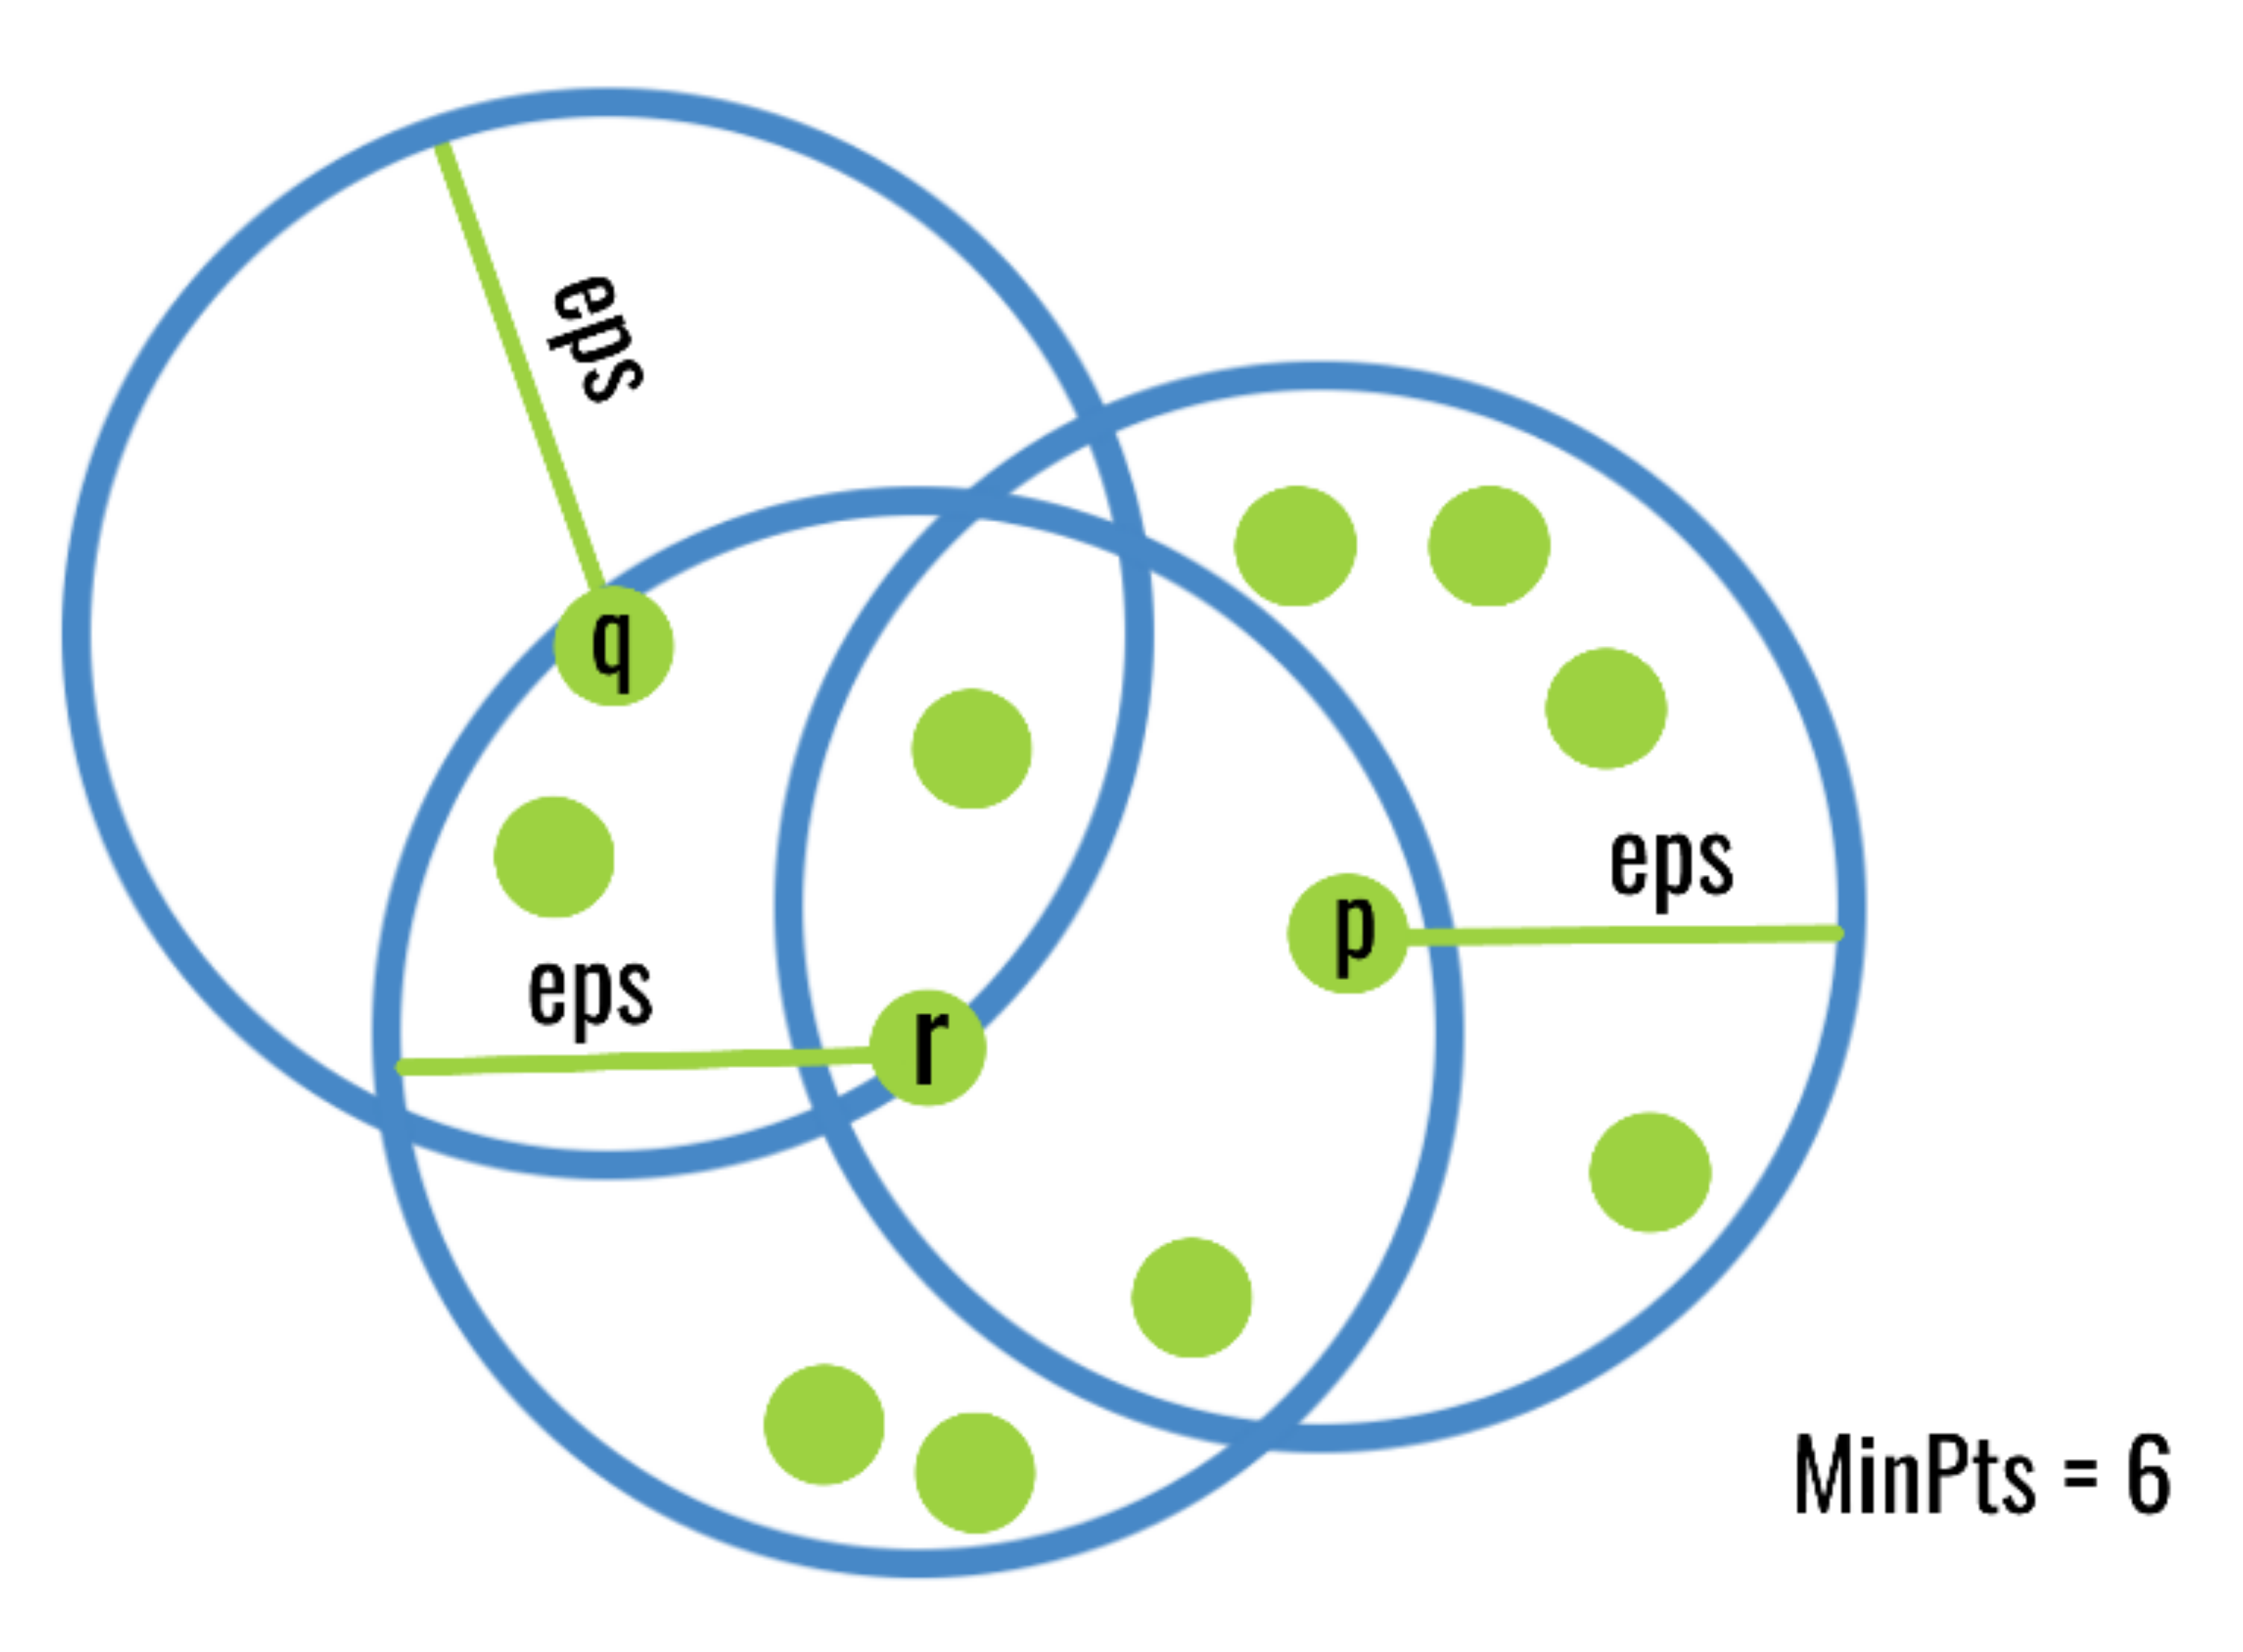
\includegraphics[width=1\textwidth]{images/dbscan2.png}
\caption{Točka $q$ je dohvatljiva iz točke $p$ preko točke $r$}
\end{subfigure}
\begin{subfigure}{.3\textwidth}
\centering
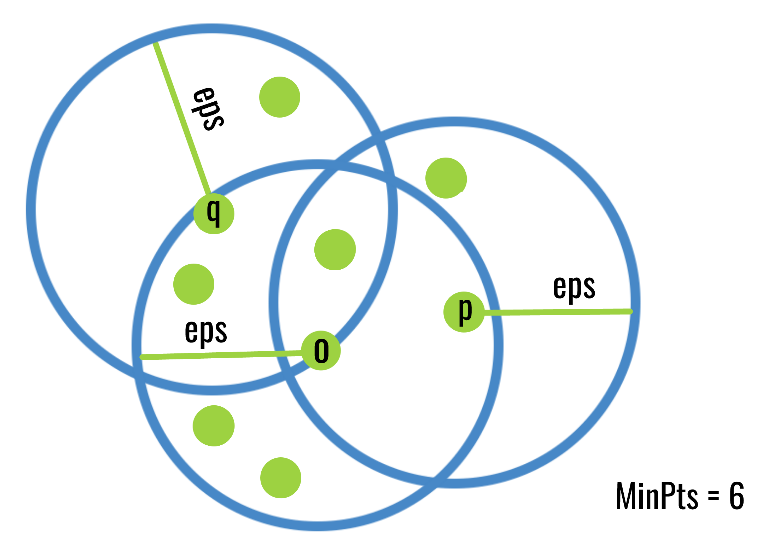
\includegraphics[width=1\textwidth]{images/dbscan3.png}
\caption{Točka $p$ i točka $q$ su povezane preko točke $o$}
\end{subfigure}
\caption{Prikaz izravne dohvatljivosti, dohvatljivosti i povezanosti na primjeru gdje je $minPts = 6$. Slike su preuzete s https://www.geeksforgeeks.org/ml-dbscan-reachability-and-connectivity/}
\label{fig:dbscan-dohvatljivost}
\end{figure}

Na početku algoritma odabire se nasumična točka od koje se formira grupa ako ona zadovoljava navedeni kriterij. Grupe se zatim rekurzivno proširuju obilaženjem ostalih članova grupe. Kad se grupa više ne može proširiti, odabire se nasumično nova točka iz skupa podataka i algoritam se ponavlja dok sve točke nisu obiđene. Pseudokod \ref{alg:dbscan} prikazuje pseudokod algoritma DBSCAN.

\begin{lstlisting}[caption = Pseudokod algoritma DBSCAN, label = {alg:dbscan}, escapeinside={*}{-}]
 definiraj minimalan broj članova grupe *$minPts$+ i udaljenost *$\epsilon$-
 inicijaliziraj početni broj grupa: *$C = 0$-
 za svaku točku *$p \in D$-
 	ako je točka *$p$- već označena
       		nastavi
    	pronađi skup točaka *$S$- izravno dohvatljivih iz *$p$-
    	ako je *$|S| < minPts$- onda 
 		označi *$p$- kao točku šuma
 	   	nastavi
 	*$C = C + 1$-
 	dodaj *$p$- u grupu *$C$-
	za svaku točku *$q \in S$-
	  	ako točka *$q$- već pripada grupi
	  		nastavi
	      	dodaj *$q$- u grupu *$C$-
	      	pronađi skup točaka *$N$- izravno dohvatljivih iz *$q$-
	      	ako je *$|N| \geq minPts$- onda 
	         	dodaj točke iz *$N$- u skup *$S$-

\end{lstlisting}

Ako je skup podataka pohranjen tako da se upiti o susjedstvu mogu izvoditi u logaritamskom vremenu, složenost DBSCAN algoritma je $O(n log n)$, gdje je $n$ broj podataka. Ako nema strukture indeksiranja, složenost raste na $O(n^2)$.

Prednosti algoritma DBSCAN su što ne zahtjeva definiranje broja grupa unaprijed, može pronaći grupe proizvoljnog oblika i otporan je na prisutnost šuma i anomalija. Nedostatak mu je što ne može dobro grupirati skup podataka u kojem je prisutna velika razlika u gustoći među grupama jer se tada ne može odabrati kombinacija parametara \textit{minPts} i $\epsilon$ koja bi bila prikladna za sve grupe. 

\section{Gaussova mješavina}

Gaussova mješavina je model distribucije koji pretpostavlja da su sve točke iz skupa podataka generirane iz mješavine konačnog broja Gaussovih distribucija s nepoznatim parametrima. Model zatim grupira podatke na način da svaka grupa sadrži podatke iz jedne distribucije.

Gaussova distribucija još se naziva normalnom distribuciju i ima karakterističan zvonolik oblik. Funkcija gustoće vjerojatnosti Gaussove distribucije u jednoj dimenziji glasi:
\begin{equation} \label{eq:gauss1}
\mathcal{N}(x|\mu,\sigma) = \frac{1}{{\sigma \sqrt {2\pi } }}e^{{{ - \left( {x - \mu } \right)^2 } \mathord{\left/ {\vphantom {{ - \left( {x - \mu } \right)^2 } {2\sigma ^2 }}} \right. \kern-\nulldelimiterspace} {2\sigma ^2 }}}
\end{equation}

pri čemu je:
\begin{itemize}
\item $\mu$ - srednja vrijednost skupa podataka; određuje ``visinu'' krivulju
\item $\sigma$ - standardna devijacija podataka; odeđuje ``širinu'' krivulje
\end{itemize}

Slika \ref{fig:gauss1} prikazuje funkciju gustoće vjerojatnosti za različite vrijednosti parametara $\mu$ i $\sigma$.

\begin{figure}[htb]
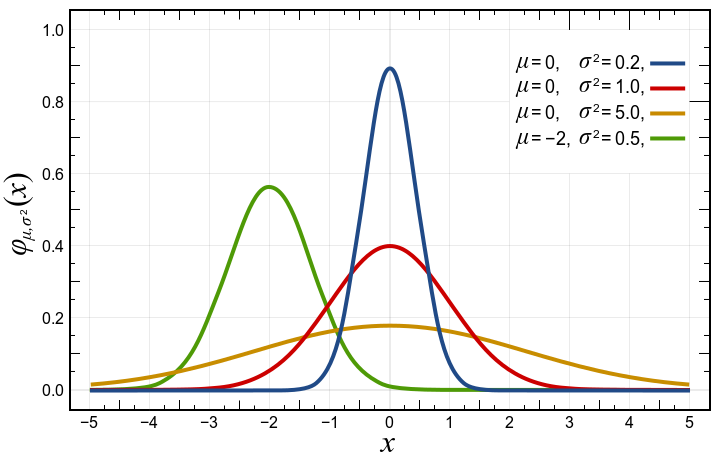
\includegraphics[width=0.8\textwidth]{images/gauss1.png}
\centering
\caption{Funkcija gustoće vjerojatnosti Gaussove distrubucije za različite vrijednosti parametara $\mu$ i $\sigma$. Preuzeto s  https://en.wikipedia.org/wiki/Normal\_distribution}
\label{fig:gauss1}
\end{figure}

U slučaju više dimenzionalnog skupa podataka, formula multivarijatna (višedimenzijske) Gaussove razdiobe glasi:

\begin{equation}
\mathcal{N}(X|\mu,\Sigma)  =\frac{1}{\sqrt{(2\pi)^{k}|\Sigma|}}exp(-\frac{1}{2}(X-\mu)^T\Sigma^{-1}(X-\mu))
\end{equation}

U tom je slučaju $k$ broj dimenzija skupa podatka, $\mu$ $k$-dimenzionalni vektor srednjih vrijednosti, a $\Sigma$ kovarijacijska matrica veličine $k \times k$.

Gaussova je mješavina funkcija koja se sastoji od onoliko Gaussovih funkcija koliko ima grupa u skupu podataka. Svaka Gaussov funkcija u mješavini ima sljedeće parametare:
\begin{itemize}
\item Srednju vrijednost $\mu$ koja definira središte.
\item Kovarijancu $\Sigma$  koja odeđuje ``širinu'' funckije.
\item Vjerojatnost miješanja $\pi$ koja definira koliko će Gaussova funkcija biti mala ili velika. Za vjerojatnosti miješanja mora vrijediti: 
\begin{equation}
\sum_{k=1}^{K}\pi_k = 1
\end{equation}
\end{itemize}

Slika \ref{fig:gauss-mixture} prikazuje kako model Gaussove mješavine grupira podatke u slučaju kada imamo tri grupe.

\begin{figure}[htb]
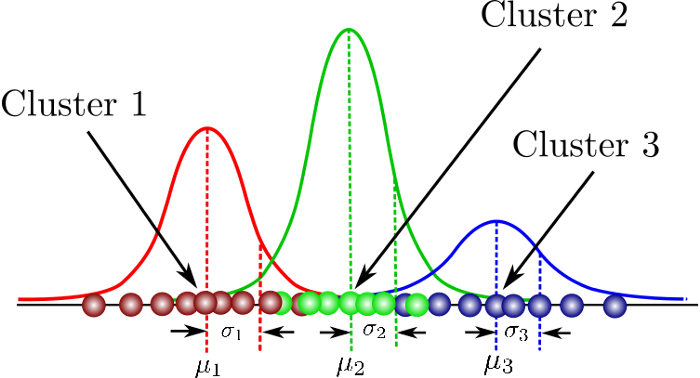
\includegraphics[width=0.8\textwidth]{images/gauss_mixture.png}
\centering
\caption{Primjer Gaussove mješavine za tri grupe podataka. Preuzeto s  https://towardsdatascience.com/gaussian-mixture-models-explained-6986aaf5a95}
\label{fig:gauss-mixture}
\end{figure}

Model Gaussove mješavine radi na principu generativnog modeliranja

Why are we using the Gaussian distribution? The Expectation-Maximization algorithm is actually more broad than just the normal distribution, but what makes Gaussians so special? It turns out that many dataset distributions are actually Gaussian! We find these Gaussians in nature, mathematics, physics, biology, and just about every other field! They are ubiquitous! There is a famous theorem in statistics called the Central Limit Theorem that states that as we collect more and more samples from a dataset, they tend to resemble a Gaussian, even if the original dataset distribution is not Gaussian! This makes Gaussian very powerful and versatile!

\chapter{Korišteni skupovi podataka}
\section{prvi}
\section{drugi}
\section{treći}

\chapter{Implementacija}

\chapter{Rezultati}







\chapter{Zaključak}
Zaključak.

\nocite{*}
\bibliography{literatura}
\bibliographystyle{fer}

\begin{sazetak}
Sažetak na hrvatskom jeziku.

\kljucnerijeci{Ključne riječi, odvojene zarezima.}
\end{sazetak}

% TODO: Navedite naslov na engleskom jeziku.
\engtitle{Title}
\begin{abstract}
Abstract.

\keywords{Keywords.}
\end{abstract}

\end{document}
